\documentclass[a4paper, oneside]{discothesis}

% use utf8 instead of latin1 when using LaTeX in windows
\usepackage[latin1]{inputenc}
\usepackage{mathtools}
\usepackage{comment}
\DeclareMathOperator*{\argmax}{\operatorname{argmax}}

%%%%%%%%%%%%%%%%%%%%%%%%%%%%%%%%%%%%%%%%%%%%%%%%%%%%%%%%%%%%%%%%%%%%%%%%%%%%%%%%%%%%%%%%%%%%%%%%%
% DOCUMENT METADATA

\thesistype{Master Thesis}
\title{Adabtive Hierarchical Deep Reinforcement Learning}

\author{Florian Frei}
\email{flofrei@student.ethz.ch}
\institute{Distributed Computing Group \\[2pt]
Computer Engineering and Networks Laboratory \\[2pt]
ETH Z�rich}

% You can put in your own logo here "\includegraphics{...}" or just comment the command
\logo{}

\supervisors{Gino Brunner, Oliver Richter\\[2pt] Prof.\ Dr.\ Roger Wattenhofer}

% You can comment the following two commands if you don't need them
% \keywords{Keywords go here.}
% \categories{ACM categories go here.}

\date{\today}

%%%%%%%%%%%%%%%%%%%%%%%%%%%%%%%%%%%%%%%%%%%%%%%%%%%%%%%%%%%%%%%%%%%%%%%%%%%%%%%%%%%%%%%%%%%%%%%%%

\begin{document}

\frontmatter % do not remove this line
\maketitle

\cleardoublepage

\begin{acknowledgements}
	I thank you.
\end{acknowledgements}


\begin{abstract}
	smart short recapitulation of stuff done
	main work experiments with temporal abstraction and their adaptability 
\end{abstract}

\tableofcontents

\mainmatter % do not remove this line

Main reference deep learning \cite{goodfellow2016deep}
Proximal Policy Approximation for OpenAI five \cite{schulman2017proximal}

\chapter{Introduction}
In 2017 an artificial intelligence named Alpha Go \cite{silver2017mastering} beat the worlds known strongest player. This was achieved without using human knowledge but rather only with playing against itself. Hence reinforcement learning has high potential to learn more complex tasks and thus help humans in the next breakthrough in technology. Maybe this comes by enabling neural networks to do temporal abstraction on its objective. Therefore in this work we want to test the adaptability and limitations of the option-critic architecture from Harb et al. (2017) \cite{harb2017waiting} and the usability of deliberation cost. 

\section*{Background}
The research topic of artificial intelligence or machine learning respectively is huge and also really old. We don't mention the basics and concentrate on the aspect of deep learning. We recommend the book from Goodfellow et al. (2016) \cite{goodfellow2016deep} as an introduction and we will assume the reader has a basic understanding of its content. Two algorithms worth mentioning is the deep Q-network(DQN) algorithm from Mnih et al. (2015) \cite{mnih2015human} and the asynchronous actor critic(A3C) from Mnih et al. (2016) \cite{mnih2016asynchronous}.

\section*{Related Work}
The idea of using a hierarchy in reinforcement learning to increase efficiency is well established. The first approach was to define macro actions or operators which can be invoked instead of just basic actions. The first three real frameworks which are still used today were proposed in the nineties. To summarize these three major frameworks were the options framework of Sutton et al. (1999) \cite{sutton1999between}, the HAM(hierarchical abstract machines) framework of Parr et al. (1998) \cite{parr1998reinforcement}, and the MaxQ framework of Dietterich (2000) \cite{dietterich2000hierarchical}. This thesis is based on the options framework.

\chapter{Preliminaries}

\section*{Markov Decision Process(MDP)}
A finite discounted MDP $\mathcal{M}$ is a tuple $\mathcal{M} \doteq (\mathcal{S},\mathcal{A},\gamma,r,P)$ encapsulating a state space $\mathcal{S}$, an action space $\mathcal{A}$, a discount factor $\gamma$ where $\gamma \in [0,1)$, a reward function $r(s,a): \mathcal{S} \times \mathcal{A} \to \mathbb{R}$ which maps a state-action pair to a real number and state transition probability function $P(s,a):\mathcal{S} \times \mathcal{A} \to \mathbb{S} $ which maps old states with actions to new states.

\section*{Policy $\pi$}
A policy $\pi(s) : \mathcal{S} \to \mathcal{A} $ is a description of behavior. Meaning in a deterministic setting the action taken is always the same given the same state. In a stochastic setting the policy $\pi(a | s) : \mathcal{S} \times \mathcal{A} \to [0,1]$ is a distribution given a state. This means an action is sampled from this distribution where each action has a probability of getting selected.

\section*{Value Function}
For each action in given state $s$ the environment returns a reward $r(s,a)$. Based on this reward value function can be defined as follows given start state $s$:
\begin{equation*}
V^{\pi}(s) = \mathbb{E} \left[ \sum_{t=1}^{\infty} \gamma^{t} r_t(s_t,a=\pi(s_t)) \right]
\end{equation*}
This value can be used to compare different policies given start state $s$. With the same concept in mind a value can be calculated when the first action is additionally separated from the rest of the policy. This yields a state-action value function $Q_{\pi}(s,a):\mathcal{S}\times\mathcal{A} \to \mathbb{R}$ which can be used to compare different initial actions $a$ from a given start state $s$.

\subsection*{$\epsilon$-greedy policy}
An $\epsilon$-greedy policy is a policy where with $\epsilon$ probability a random action is taken:
\begin{equation*}
\pi_{\epsilon}
\end{equation*}
Most theory of reinforcement learning research is based on Markov Decision Processes(MDP) since it provides the simplest framework which allows us to study basic algorithms and their properties. A finite discounted MDP $\mathcal{M}$ is a tuple $\mathcal{M} \doteq (\mathcal{S},\mathcal{A},\gamma,r,P)$ encapsulating a state space $\mathcal{S}$, an action space $\mathcal{A}$, a discount factor $\gamma$ where $\gamma \in [0,1)$, a reward function $r(s,a): \mathcal{S} \times \mathcal{A} \to \mathbb{R}$ which maps a state-action pair to a real number and state transition probability function $P(s,a):\mathcal{S} \times \mathcal{A} \to \mathbb{S} $ which maps old states with actions to new states.\\
A policy $\pi(s) : \mathcal{S} \to \mathcal{A} $ is a description of behavior. Meaning in a deterministic setting the action taken is always the same given the same state. In a stochastic setting the policy $\pi(a | s) : \mathcal{S} \times \mathcal{A} \to [0,1]$ is a distribution given a state. This means an action is sampled from this distribution where each action has a probability of getting selected.


\section*{Option-critic}
This is needed since options in the options framework from Sutton et al. (1999) \cite{sutton1999between} depend on past decisions. Options are in essence encapsulated policies and thus also a super-policy is required who decides which options gets control in a given state. The last piece needed is a function which describes when a sub-policy should terminate itself and give control back to the super-policy. Mathematically described an option consists of three components. A stochastic sub-policy $\pi_{\omega}:\mathcal{S}\times \mathcal{A} \to [0,1]$ which represents the behavior of an option $\omega$, a termination function $\beta: \mathcal{S} \to [0,1]$ which describes the probability of terminating option $\omega$ given state $s$, and an initiation set $\mathcal{I}_{\omega} \subset \mathcal{S}$ containing the all states from which an option $\omega$ can start from. Last but not least the super-policy $\pi_{\Omega}: \mathcal{S} \times \Omega \to [0,1]$ where $\Omega$ is the set of options. The super-policy can again be an $\epsilon$-greedy policy.\\%but now we act greedily based on the estimated $Q$-value belonging to the options. 
\includegraphics[scale=1.3]{option_critic_arch.pdf}\\
The option-critic architecture is similar to the actor-critic algorithm hence the name. For a complete mathematical derivation we refer to Bacon et al. (2017) \cite{bacon2017option} where everything can be found and we only highlight the resulting equations. In this architecture the super-policy acts $\epsilon$-greedy based on $Q$-values learned by $Q$-learning. The super-policy selects an option which is as already mentioned just a stochastic sub-policy and returns basic actions until termination. As one can imagine this model allows in a sense temporally extended sub-strategies. When the termination function is to high for all states the algorithm collapses to basic actions but chosen indirectly over options. The initiation set is generally given by the set of all states meaning any option can start from any state. The function for the $Q$-values used by the super-policy is given by the following equation:
\begin{equation*}
Q_{\Omega}(s,\omega) = \sum_{a} \pi_{\omega,\theta}(a|s) Q_{U}(s,\omega,a)
\end{equation*}
It is simply the expectation over all actions an option $\omega$ can take and a corresponding state-option-action value given by the sub-policy. The state-option-action value function is defined as follows:
\begin{gather*}
Q_{U}(s,\omega,a) = r(s,a) + \gamma \sum_{s'} P(s'|s,a) U(\omega,s') \\
U(\omega,s') = (1-\beta_{\omega,\vartheta}(s'))Q_{\Omega}(s',\omega) + \beta_{\omega,\vartheta}(s') V_{\Omega}(s')
\end{gather*}
where $U(\omega,s')$ is an utility term calculated for the two cases. When the option $\omega$ does not terminate we use the $Q$-value from before for the new state $s'$ otherwise use an estimation $V_{\Omega}(s')$ over all options. Note that this recursion has the same structure as the Bellman equation and hence TD estimation is also applicable. The derivation is the same as before by taking the gradients with respect to $\theta$ and $\vartheta$ as to maximize the expected return for all states. 

\subsection*{Intra-option gradient}
First we show the policy gradient of the sub-policies also called intra-option gradient. 

\begin{gather*}
\rho(\theta) = \mathbb{E}\left[  \sum_{t=1}^{\infty} \gamma^{t-1} R_t \bigg| s_0,\omega_0,\Omega \right]=Q_{\Omega}(s_0,\omega_0) \\
\frac{\partial Q_{\Omega}(s,\omega) }{\partial \theta} = \sum_{s} \sum_{\omega} d_{\Omega}(s,w) \sum_{a} \frac{\partial \pi_{\omega,\theta}(a|s) }{\partial \theta } Q_{U}(s,\omega,a)
\end{gather*}
Note that here the same old trick with the log transformation and using action sampling can be made. Also $d_{\Omega}(s,w)$ is again the discounted weighting of states along an option.

\subsection*{Termination gradient}
Next is the gradient from the termination where we want to maximize the utility function. 
\begin{gather*}
\rho(\vartheta) = \mathbb{E}\left[  \sum_{t=1}^{\infty} \gamma^{t-1} R_t \bigg| s',\omega,\Omega \right]=U(s',\omega) \\
\frac{\partial U_{\omega, s'} }{\partial \vartheta} = \sum_{\omega'} \sum_{s''} d_{\Omega}(s',\omega ) \frac{\partial \beta_{\omega',\vartheta}(s'') }{\partial \vartheta} \left( V_{\Omega}(s'') - Q_{\Omega}(s'',\omega') \right)
\end{gather*} 
where $A_{\Omega}(s',\omega) = Q_{\Omega}(s',\omega')- V_{\Omega}(s') $ is the already seen advantage function with respect to option $\omega$. This makes intuitively sense because $V_{\Omega}(s')$ is estimated from all options. Hence when there is a better option this value is higher than the current state-option value and the advantage function is negative. Thus the sum is positive and we increase the termination probability. The same logic applies for the reverse case where we want to decrease the termination probability in case the state-option value is higher than value estimation from all options. \\
In case that the action space is to large and therefore $N_{\Omega} \cdot N_{\mathcal{A}}$ huge we can estimate $Q_U$ from $Q_{\Omega}$ as shown below:
\begin{equation*}
Q_{U}(s,\omega,a) = r(s,a) + \gamma \sum_{s'} P(s'|s,a) U(\omega,s')=r(s,a)+\gamma \mathbb{E}_{s' \sim P } \left[ U(\omega,s') \big| s,a \right]
\end{equation*}
\TODO{pseudo code for option critic?}

\section*{Deliberation cost}


\begin{comment}
% Start writing here
\chapter{Motivation}
The human capability to learn abstract concepts is well-known but not well understood. Our brain is the most complex organ in our body and its size is the most significant difference to other species. It allows us to be self-aware and defines our individuality. Hence it could be of significant importance to understand how it works for creating artificial intelligence. One aspect of it is the brains capability of high level abstraction. This could be temporal or objective in nature. Meaning that we learn automatically to tackle difficult tasks by dividing them into manageable subtasks. Additionally the function of dopamine allows us to handle delayed gratification. Meaning that for example no immediate reward is needed for pursuing a goal in life. The journey is a sufficient inner motivator regardless if we can reach the set goal. The high complexity of games in the world today such as League of Legends, Dota 2 or Starcraft require a more sophisticated abstraction of the strategy in order to win. Recently they achieved more than human level performance in Dota 2 with training a neural network over half a year but no abstraction levels were used. Thus it is important to better understand abstraction such that it is possible to incorporate abstraction into neural networks to allow better performance. 

\chapter{Introduction}
%Reinforcment Learning
\section*{Reinforcement Learning}
Reinforcement Learning(RL) is besides supervised and unsupervised learning one of the big three themes in machine learning. Without going into details this research field is mostly based on the theory of Markov Decision Processes. There are other types of approaches worth mentioning but we don't want to go into to much detail. For the interested reader or for a complete beginner in this kind of field we refer to we refer Sutton et al. (1998) \cite{sutton1998introduction} and Kaelbling et al. (1996) \cite{kaelbling1996reinforcement} where most on theory and history of this research field with all references can be found.\\
In this work we concentrate on one subfield of reinforcement learning namely hierarchical reinforcement learning. We think a good start where most frameworks are well summarized is in Barto et al.(2003) \cite{barto2003recent} and it also gives a brief introduction to the theory of Markov Decision Processes abbreviated as MDP. For the interested reader which is not particularly fond of reading papers we refer to video course by David Silver free available online on youtube.

\section*{Hierarchical Reinforcement Learning}
%Hierarchical reinforcement learning
The idea of using a hierarchy in reinforcement learning to increase efficiency is well established. The first approaches was to define macro actions or operators which can be invoked instead of just basic actions. The first three real frameworks which are still used today were proposed in the nineties. To summarize these three major frameworks were the options framework of Sutton et al. (1999) \cite{sutton1999between}, the HAM(hierarchical abstract machines) framework of Parr et al. (1998) \cite{parr1998reinforcement}, and the MaxQ framework of Dietterich (2000) \cite{dietterich2000hierarchical}. This thesis is based on the options framework and hence we concentrate only on this type of framework but this does not mean the others are not worth consideration.

\section*{Deep Reinforcement Learning}
Another big aspect in the development of machine learning is due to the rapid improvement of the hardware. More memory and CPU capacity allows faster exploration and tackling more complex tasks. This allowed the realization of neural networks and hence the field of deep reinforcement learning. For a reader which never heard of neural networks we refer to Funahashi (1989) \cite{funahashi1989approximate} where the theory and research references can be found. Neural networks form the basis of most deep reinforcement algorithms today and are used extensively. 

%Bad start reference to randomly sampled replay buffer in RL
%A good starting point into this topic is the work of Mnih et al. (2015) \cite{mnih2015human} which shows that a high level of control can be achieved. 
The state of the art algorithm A3C(asynchronous advantage actor critic) can be found in Mnih et al.(2016) \cite{mnih2016asynchronous} which is often used as a baseline to compare the performance of new developed techniques and algorithms.

% The toolkit we use to compare algorithms fairly on different environments is given by the OpenAI gym from Brockman et al. \cite{brockman2016openai} and will be used as a base in this work to implement our own environments. \\
%To implement neural networks we refer to two libraries namely the overworked theano framework \cite{bergstra2011theano} from Bastien et al. (2012) \cite{bastien2012theano} and tensorflow from Abadi et al. (2016) \cite{abadi2016tensorflow}. In this work we will exclusively use tensorflow in python.
%In this work we concentrate on the proposed hybrid algorithm between the options framework and asynchronous advantage actor critic named option critic from \cite{harb2017waiting} where a deliberation cost was additionally introduced.

\chapter{Preliminaries}
%For the complete theory on MDP's we refer to the literature.
\section*{Markov Decision Process}
Most theory of reinforcement learning research is based on Markov Decision Processes(MDP) since it provides the simplest framework which allows us to study basic algorithms and their properties. A finite discounted MDP $\mathcal{M}$ is a tuple $\mathcal{M} \doteq (\mathcal{S},\mathcal{A},\gamma,r,P)$ encapsulating a state space $\mathcal{S}$, an action space $\mathcal{A}$, a discount factor $\gamma$ where $\gamma \in [0,1)$, a reward function $r(s,a): \mathcal{S} \times \mathcal{A} \to \mathbb{R}$ which maps a state-action pair to a real number and state transition probability function $P(s,a):\mathcal{S} \times \mathcal{A} \to \mathbb{S} $ which maps old states with actions to new states.\\
A policy $\pi(s) : \mathcal{S} \to \mathcal{A} $ is a description of behavior. Meaning in a deterministic setting the action taken is always the same given the same state. In a stochastic setting the policy $\pi(a | s) : \mathcal{S} \times \mathcal{A} \to [0,1]$ is a distribution given a state. This means an action is sampled from this distribution where each action has a probability of getting selected.

\section*{Value Function}
Since a reward can be assigned to each state a value function can be calculated from start state $s$ with a given stochastic policy as follows:
\begin{equation*}
V^{\pi}(s) = \mathbb{E} \left[ \sum_{t=1}^{\infty} \gamma^{t} r_t(s_t,a=\pi(s_t)) \right]
\end{equation*}
This value can be used to compare different policies given start state $s$. With the same concept in mind a value can be calculated when the first action is additionally separated from the rest of the policy. This yields a state-action function $Q_{\pi}(s,a):\mathcal{S}\times\mathcal{A} \to \mathbb{R}$ which can be used to compare different initial actions $a$ from a given start state $s$.

\section*{Bellman Equation}
Now instead looking at the whole trajectory of a policy the Bellman equation \eqref{eq:bellman} from \cite{bellman1956dynamic} (1956) allows one to view it in a recursive manner using the value function as follows:
\begin{equation}
\label{eq:bellman}
V^{\pi} (s)= r(s,a=\pi(s)) + \gamma \sum_{s' \in \mathcal{S}}^{}{ P(s'|s,a=\pi(s)) V^{\pi}(s') }
\end{equation}
In the stochastic setting when the policy follows a distribution and every event is possible the equation can be rewritten as follows:
\begin{equation}
\label{eq:bellman2}
V^{\pi} (s)= \sum_{a}^{}{\pi(a | s)} \left( r(s,a) + \gamma \sum_{s'}^{}{ P(s'|s,a) V^{\pi}(s') } \right) 
\end{equation}
This equation was already usable in dynamic programming. Two major algorithms using Bellman equation were value iteration and policy iteration from Howard (1964) \cite{howard1964dynamic} which could solve successfully MDP's. In value iteration the algorithm acts under an implicit policy such as $\epsilon$-greedy for example and the value function is learned through the state-action function. 
\begin{gather*}
Q_{t+1}(s,t) = r(s,a) + \gamma \sum_{s'}^{}{P(s'|s,a)V_{t}(s)} \\
V_{t+1}(s) = \max_{a} Q_{t+1}(s,a)
\end{gather*}
Whereas in policy iteration a random policy $\pi$ is initialized and then learned stepwise using the value function but not the state-action function.
\begin{gather*}
V^{\pi_t}_{t+1}(s) = r(s,\pi_t(s))+\gamma \sum_{s' \in \mathcal{S}}^{}{P(s'|s,\pi_t(s))V^{\pi_t}_{t+1}(s')}\\
\pi_{t+1}(s) = \argmax_{a} \left( r(s,a) + \gamma \sum_{s'}^{}{P(s'|s,a)V^{\pi_t}_{t+1}(s')} \right)
\end{gather*}

\section*{Temporal Difference}
As one can imagine in reinforcement learning the Bellman equation allows different lengths of recursion. An algorithm using the whole trajectory in an environment are categorized under Monte Carlo methods. The alternative is Temporal Difference (TD) \cite{sutton1988learning} methods which use the Bellman equation and instead of calculating the expectation they estimate the difference from sampling. Hence the temporal difference error resulting is written as:
\begin{equation*}
\operatorname{TD}(0) = R(s,\pi(s))+\gamma V_{\pi}(s') -\gamma V_{\pi}(s) 
\end{equation*}
Notice that $s'$ was sampled from the transition probabilities and can be looked at as a zero order scheme. One can repeat the process and use the same equation to approximate the next value $V_{\pi}(s')$ and so forth. Thus arbitrary recursion schemes can be chosen for this approximation which is a design decision depending on the environment or problem respectively.

\section*{On-policy vs off-policy}
In this recursion we only talked about improving the value function but we are also interested in improving the policy $\pi$ along the way. This can be done in two manners namely on-policy or off-policy. On-policy means that only one policy is used and directly improved with the environment. Off-policy means that there are two policies. One used for exploration with generates data whereas the other policy uses this data to improve itself. Since the policies have different acting distributions sampling methods like importance sampling has to be used to eliminate bias from the action and state samples. This means that in the off-policy case an experience buffer is filled with transitions and then sampled from it to improve the policy.

\section*{SARSA and Q-Learning}
An example for an on-policy algorithm is SARSA \cite{rummery1994line} which stands abbreviated for state action reward state action meaning it uses one transition and the next action to approximate the TD-error. The policy used is $\epsilon$-greedy based on the state-action function $Q$. Meaning with probability $\epsilon$ a random action is taken otherwise the action with the maximum $Q$-value is used. The counterpart to SARSA using off-policy updates is Q-Learning \cite{watkins1992q}.

\section*{REINFORCE}
As we have seen either $\epsilon$-greedy policy was used based on action-value function $Q(s,a)$ to act or another entire policy based on experience. The functions $V(s)$ and $Q(s,a)$ helped to decide which actions are better in the environment in given state and hence improve the policy. But the policy also can be learned directly and are named policy gradient methods. The first method introduces was REINFORCE from Williams (1992) \cite{williams1992simple} where a whole trajectory like in the Monte Carlo method was utilized to improve the policy. The objective is still to maximize the expected cumulative reward.
\begin{equation*}
\rho(s) = \mathbb{E} \left[ \sum_{t=1}^{\infty}{\gamma^{t-1} R_t \Bigg| s} \right]
\end{equation*}
When we define $\tau$ as a complete trajectory and $R(\tau)$ as the reward corresponding to this trajectory the equation can be reformulated as:
\begin{equation*}
\rho(s) = \sum_{\tau}^{}{P_{\theta}(\tau) R(\tau)}
\end{equation*}
where $\theta$ represent the parameters of our policy $\pi$. Instead of using the whole trajectory one can again use an value estimation. This can be learned with TD and reformulated as maximizing:
\begin{equation*}
\rho(s) = \mathbb{E} \left[ \sum_{t=1}^{\infty}{\gamma^{t-1} R_t \Bigg| s} \right] = \sum_{a}^{}{\pi(a|s)Q^{\pi}(s,a)=V^{\pi}(s)}
\end{equation*}
We will not go into detail for the derivation and refer to Sutton et al. (2000) \cite{sutton2000policy} and just present the resulting gradient.
\begin{equation*}
\frac{\partial V^{\pi}(s)}{\partial \theta} = \sum_{x}^{}{d^{\pi}(x)} \sum_{a}^{}{\frac{\partial \pi(a|x) }{\partial \theta} Q^{\pi}(x,a)} 
\end{equation*}
where $d^{\pi}(s)$ is defined as the discounted weighting of states encountered starting at some state $s_0$. In practice most algorithms use $d^{\pi}(x)$ as a stationary distribution which results in an expectation over states. Additionally a baseline is added to reduce variance and together with the log transformation trick the sum can be reduced as follows:
\begin{gather*}
\frac{\partial V^{\pi}(s)}{\partial \theta} = \sum_{s}^{} d^{\pi}(s) { \sum_{a}^{} { \frac{\partial \pi(a|s) }{\partial \theta}  \left[ Q^{\pi}(s,a) - V(s) \right] } } \\
=\sum_{s}^{}{d^{\pi}(s)} \mathbb{E} \left[  \frac{\partial \log{ \pi(a|s) } }{\partial \theta} \left( Q^{\pi}(s,a) - V(s) \right) \right]
\end{gather*}
Note that $V(s)$ in the expectation does not contribute anything so $A(s,a) = Q^{\pi}(s,a) - V(s)$ is often used and known as advantage function. 

\section*{Actor-critic}
The actor-critic algorithm is composed of an actor which learns a policy and a critic which learns a value function. The policy is learned similar to REINFORCE but learned with the value function instead of a sample trajectory. The value function off the current policy is learned via TD approximation. The resulting equations are listed below.  
\begin{gather*}
\frac{\partial \rho}{\partial \vartheta} = \sum_{s} d^{\pi}(s) \sum_{a} \frac{\partial \pi(s,a)}{\partial \vartheta } Q^{\pi}(s,a)= \sum_{s} d^{\pi}(s) \mathbb{E}_a \left[  \frac{\partial \log(\pi(a|s) ) }{\partial \vartheta } Q^{\pi}(s,a) \right] \\
\frac{\partial Q(s,a)}{\partial \theta} = \frac{\partial \left( R(s,a) + \gamma \mathbb{E}_{s'\sim P(s'|s,a)}[V(s')]-Q(s,a) \right)^2 }{\partial \theta} = - \sigma \ast \frac{\partial Q(s,a)}{\partial \theta}
\end{gather*}

\includegraphics[scale=1.3]{actor_critic_arch.pdf}

The next step is to incorporate temporal abstraction into an algorithm. This is no longer possible with simple MDP's and thus the concept was generalized to Semi Markov Decision Processes(SMPD) and we refer to \cite{puterman2014markov} for further reading.

\TODO{SMPD graphic}

\section*{Option-critic}
This is needed since options in the options framework from Sutton et al. (1999) \cite{sutton1999between} depend on past decisions. Options are in essence encapsulated policies and thus also a super-policy is required who decides which options gets control in a given state. The last piece needed is a function which describes when a sub-policy should terminate itself and give control back to the super-policy. Mathematically described an option consists of three components. A stochastic sub-policy $\pi_{\omega}:\mathcal{S}\times \mathcal{A} \to [0,1]$ which represents the behavior of an option $\omega$, a termination function $\beta: \mathcal{S} \to [0,1]$ which describes the probability of terminating option $\omega$ given state $s$, and an initiation set $\mathcal{I}_{\omega} \subset \mathcal{S}$ containing the all states from which an option $\omega$ can start from. Last but not least the super-policy $\pi_{\Omega}: \mathcal{S} \times \Omega \to [0,1]$ where $\Omega$ is the set of options. The super-policy can again be an $\epsilon$-greedy policy.%but now we act greedily based on the estimated $Q$-value belonging to the options. 

\includegraphics[scale=1.3]{option_critic_arch.pdf}

The option-critic architecture is similar to the actor-critic algorithm hence the name. For a complete mathematical derivation we refer to Bacon et al. (2017) \cite{bacon2017option} where everything can be found and we only highlight the resulting equations. In this architecture the super-policy acts $\epsilon$-greedy based on $Q$-values learned by $Q$-learning. The super-policy selects an option which is as already mentioned just a stochastic sub-policy and returns basic actions until termination. As one can imagine this model allows in a sense temporally extended sub-strategies. When the termination function is to high for all states the algorithm collapses to basic actions but chosen indirectly over options. The initiation set is generally given by the set of all states meaning any option can start from any state. The function for the $Q$-values used by the super-policy is given by the following equation:
\begin{equation*}
Q_{\Omega}(s,\omega) = \sum_{a} \pi_{\omega,\theta}(a|s) Q_{U}(s,\omega,a)
\end{equation*}
It is simply the expectation over all actions an option $\omega$ can take and a corresponding state-option-action value given by the sub-policy. The state-option-action value function is defined as follows:
\begin{gather*}
Q_{U}(s,\omega,a) = r(s,a) + \gamma \sum_{s'} P(s'|s,a) U(\omega,s') \\
U(\omega,s') = (1-\beta_{\omega,\vartheta}(s'))Q_{\Omega}(s',\omega) + \beta_{\omega,\vartheta}(s') V_{\Omega}(s')
\end{gather*}
where $U(\omega,s')$ is an utility term calculated for the two cases. When the option $\omega$ does not terminate we use the $Q$-value from before for the new state $s'$ otherwise use an estimation $V_{\Omega}(s')$ over all options. Note that this recursion has the same structure as the Bellman equation and hence TD estimation is also applicable. The derivation is the same as before by taking the gradients with respect to $\theta$ and $\vartheta$ as to maximize the expected return for all states. 

\subsection*{Intra-option gradient}
First we show the policy gradient of the sub-policies also called intra-option gradient. 

\begin{gather*}
\rho(\theta) = \mathbb{E}\left[  \sum_{t=1}^{\infty} \gamma^{t-1} R_t \bigg| s_0,\omega_0,\Omega \right]=Q_{\Omega}(s_0,\omega_0) \\
\frac{\partial Q_{\Omega}(s,\omega) }{\partial \theta} = \sum_{s} \sum_{\omega} d_{\Omega}(s,w) \sum_{a} \frac{\partial \pi_{\omega,\theta}(a|s) }{\partial \theta } Q_{U}(s,\omega,a)
\end{gather*}
Note that here the same old trick with the log transformation and using action sampling can be made. Also $d_{\Omega}(s,w)$ is again the discounted weighting of states along an option.

\subsection*{Termination gradient}
Next is the gradient from the termination where we want to maximize the utility function. 
\begin{gather*}
\rho(\vartheta) = \mathbb{E}\left[  \sum_{t=1}^{\infty} \gamma^{t-1} R_t \bigg| s',\omega,\Omega \right]=U(s',\omega) \\
\frac{\partial U_{\omega, s'} }{\partial \vartheta} = \sum_{\omega'} \sum_{s''} d_{\Omega}(s',\omega ) \frac{\partial \beta_{\omega',\vartheta}(s'') }{\partial \vartheta} \left( V_{\Omega}(s'') - Q_{\Omega}(s'',\omega') \right)
\end{gather*} 
where $A_{\Omega}(s',\omega) = Q_{\Omega}(s',\omega')- V_{\Omega}(s') $ is the already seen advantage function with respect to option $\omega$. This makes intuitively sense because $V_{\Omega}(s')$ is estimated from all options. Hence when there is a better option this value is higher than the current state-option value and the advantage function is negative. Thus the sum is positive and we increase the termination probability. The same logic applies for the reverse case where we want to decrease the termination probability in case the state-option value is higher than value estimation from all options. \\
In case that the action space is to large and therefore $N_{\Omega} \cdot N_{\mathcal{A}}$ huge we can estimate $Q_U$ from $Q_{\Omega}$ as shown below:
\begin{equation*}
Q_{U}(s,\omega,a) = r(s,a) + \gamma \sum_{s'} P(s'|s,a) U(\omega,s')=r(s,a)+\gamma \mathbb{E}_{s' \sim P } \left[ U(\omega,s') \big| s,a \right]
\end{equation*}
\TODO{pseudo code for option critic?}

\subsection*{Regularization}

As often used in state of the art algorithms some regularization is added to some gradients. This can prevent over-fitting to a local optimum by adding randomness to actions such as in entropy regularization. In regard to the termination gradient a small constant term is added since using $\epsilon$-greedy super-policy leads mostly to termination probability of 100\%. This is caused by the value function since
\begin{gather*}
V(s) = \displaystyle \max_{\omega} Q_{\Omega}(s',\omega)
\intertext{and hence}
Q_{\Omega }(s',\omega) - \max_{\omega} Q_{\Omega}(s',\omega) \leq 0 \\
\intertext{and thus the new termination gradient is given by}
\frac{ \partial \beta_{\omega,\vartheta(s')} }{\partial \vartheta} \left( Q_{\Omega}(s',\omega) - \max_\omega Q_\Omega(s,\omega) + \eta_\beta \right)
\end{gather*}
and therefore we allow $\eta_\beta$ margin error between the maximum $Q$-value and the current one given with option $\omega$. As already mentioned there could be a problem with the options where their policy get stuck in a deterministic action distribution. To counter this behavior an entropy is added to the intra-option gradient as shown in the A3C algorithm in Mnih et al. (2016) \cite{mnih2016asynchronous} The entropy is calculated as follows:
\begin{gather*}
H( \pi_{\omega,\theta}(\cdot |s) ) = -\sum_{a} \pi_{\omega,\theta}(a|s)\log(\pi_{\omega,\theta}) \\
\intertext{And hence the new gradient has the following form:}
\frac{\partial Q_{\Omega}(s,\omega) }{\partial \theta} = \frac{\partial \log(\pi_{\omega,\theta}(a|s) )}{\partial \theta} Q_U(s,\omega,a) + \eta_H \cdot \frac{\partial H( \pi_{\omega,\theta}(\cdot |s) )}{\partial \theta}
\end{gather*}

\subsection*{Deliberation Cost}

\TODO{graphic from paper}


\chapter{Implementation}
\end{comment}

\section*{Implementation details}

We based our implementation on the UNREAL \cite{miyoshigithubunreal} implementation of Jaderberg et al. (2016) \cite{jaderberg2016reinforcement} which uses the Asynchronous Advantage Actor Critic(A3C) algorithm from Mnih et al (2016) \cite{mnih2016asynchronous}. Next we implemented Asynchronous Advantage Option Critic(A2OC) from Harb et al. (2017) \cite{harb2017waiting} where a theano based implementation can be found here \cite{harbgithuba2oc}.

\subsection*{Environment}
Most interesting learn environments used such as the Arcade Learning Environment (ALE) \cite{brockman2016openai} or the DeepMind Lab \cite{beattie2016deepmind} where complicated tasks are learned from pixel inputs are harder to study. The simple reason is that the network heavily relies on GPU's and their ability to fast transform pixel inputs in the convolution layer to features usable for training. Hence the training time until reasonable performance can easily take days. This is unsuitable for scientific analysis of the algorithm where we want to study the effect of each small change in the model, hyper-parameters or environment. Therefore since we repeat all simulation very often we want fast convergence. Thus we implemented simple grid worlds where we can easily control the world size and hence the input dimension to the network. The OpenAI gym toolkit from Brockman et al. \cite{brockman2016openai} allowed easy implementation of our grid-world through inheritance of their environment classes. Also there is a tutorial online on github which explains how to accomplish that.

\subsection*{Multithreading}
We used an on-policy approach where multiple threads like in Mnih et al. \cite{mnih2016asynchronous} make small batches of data, apply the gradients from this data then resynchronize the networks. For this we used the python multiprocessing tools namely Process and Pipe. This handled multiple instances of the same environments and their communication and was used in the UNREAL implementation. Since multiple threads also have their own instances of the neural networks the total resulting graph is relatively huge.


\TODO{input the graphic for graph}

\subsection*{Neural Networks}
To implement all neural networks we used the well-established tensorflow library from Abadi et al. (2016) \cite{abadi2016tensorflow} in python. In essence tensorflow constructs a direct acyclic graph for the flow of information through the layers. Elements in this graph are variables such as weights and biases but also all operations such as multiplication and addition. The nice thing about that is that the library takes care for computing backwards and forwards propagation within the network since it computes and applies the gradients itself. When $N_{\omega}$ is the number of options then we needed $N_{\omega}+3$ networks. Each options has its own neural network and hence we can test mixed models of different depth against each other. The rest is used for the termination model, the $Q$-value model and the convolution layer. Before the input gets fed into the convolution layer the input is rescaled to $[0,1]$.

\includegraphics[scale=0.74]{option_critic.pdf}

\subsection*{Convolution network}
Since our world is relatively simple we choose one layer of convolution followed by two fully connected layers. The number of filters we choose was $64$ and the filter size was chosen the same as the world size. Meaning a $4 \times 4$ grid world gets a $4 \times 4$ filter since we didn't wanted to loose any information. We used padding such that the dimension stays the same meaning an input of $4 \times 4$ gets transformed to an output of $4 \times 4 \times 64$. For initialization the standard Xavier initializer for weights and Zero initializer for biases were used. For both fully connected layers Rectified Linear Units(ReLUs) were utilized as activation functions. The second fully connected layer has a dimension of $32$ units. 

\subsection*{Options network}
We utilize different deep networks of options depending on the experiment. The input comes from the convolution layer and the output is fixed to the number of possible actions. Since we use stochastic policies we need a probability vector as output which is simple achieved by using softmax as the activation function. First type was just using a bias term in the network. Meaning the output of the network is input independent. This makes sense when we want to test if everything is learnable using only the super-policy. The next type of network is adding the weights and hence is a linear combination of features. Both weights and biases are standard initialized with Xavier or Zero initializers. The last type is generated by adding one more layer with a Rectified Linear Unit as activation function with $16$ units.

\subsection*{Q-value network}
As already talked about the $Q$-value model is the basis for the super-policy for making decisions. Our $Q$-value  network has two layers. First a fully connected layer compromised of $16$ units with a ReLU activation function followed by a second fully connected layer but with a linear activation function since we have to allow negative $Q$-values for the algorithm to work properly. Whereas the output dimension is the number of options $N_{\Omega}$ since we compare among them for making decisions. 

\subsection*{Termination network}
The termination network is exactly the same as the $Q$-value network where the only difference is that the last activation is no longer linear but a sigmoid function. This gives us a vector of termination probabilities corresponding to the options. It was observed already in \cite{harb2017waiting} that the termination model suffers under over-fitting hence the introduction of a deliberation cost as a form of regularization is sensible.  


\subsection*{Sensitivity of reward function}
The convergence of the network respectively the algorithm is dependent on the reward function. First of all to avoid problems the reward functions in most cases is scaled to $[-1,1]$. Furthermore one tries to eliminate all local optima in a sensible reward function otherwise the network can get stuck during learning. It could also happen that a flaw in the reward function can lead to reward hacking and the system learns something the user never intended to. Hence constructing a sensible reward function is not an easy task. In our environment we get a reward for each step. We divided this into three categories namely stepping outside of the world, stepping inside the world, and stepping on the goal. The reward for the goal is constant $1$ and the episode is terminated. The other two have more variability and hence we want to test different scenarios. These are summarized in the table below:\\
\begin{tabular}{cccc}
Name&\{outside,flag\}&\{inside,flag\}&\{goal,flag\} \\
$S_1=$ & \{-1,True\} &\{0,False\} & \{1,True\} \\
$S_2=$ & \{-1,True\}& \{-0.1,False\}& \{1,True\} \\
$S_3=$ & \{0,True\}& \{0,False\}& \{1,True\} \\
$S_4=$ & \{-1,False\} &\{0,False\} & \{1,True\} \\
$S_5=$ & \{-1,False\}& \{-0.1,False\}& \{1,True\} \\
$S_6=$ & \{0,False\}& \{0,False\}& \{1,True\} \\
$S_7=$ & \{-0.1,False\}& \{-0.1,False\}& \{1,True\} 
\end{tabular}


As one can see the sets $S_1$ and $S_2$ have local optima. Note that in $S_2$ the local optima occurs when the agent makes more the $10$ steps in the world which is worse than walking into a wall since this terminates the episode. Furthermore when whole trajectories are used to learn like in Monte Carlo, utilizing the sets $S_4$ and $S_5$ as rewards lead with high probability that the network will not converge. Later on we introduce an additional barrier namely a key which has to picked up first before reaching the goal is possible. Picking up the key gives \{0,False\} or \{1,False\} reward and could potentially add a local optima.

\subsection*{Epsilon annealing vs. constant epsilon}
Since we use an $\epsilon$-greedy super-policy we are confronted with the question which value is reasonable. We tested two scenarios and looked at their development. First scenario is were start with the highest value of $\epsilon = 1.0$ and then anneal epsilon linearly down to $0.1$ or $0.01$ over constant number of steps. The second scenario is to let be epsilon constant $\epsilon=0.1$ or $\epsilon=0.01$ and hope that this randomness is enough over long time for convergence. 

\subsection*{Deliberation cost annealing}
The deliberation cost is mainly used to steer the termination network. For example when the termination get stuck on 0\% or 100\% but it is a local optima instead of restarting the networks the deliberation cost can be used to increase or decrease termination. 

\TODO{graphic stuck optima from paper}  


\subsection*{Exponential window function}
The tensorboard tool given with tensorflow library allows to view all defined summaries in the web-browser. This is useful for observing a current running experiment. It case something goes wrong with the network we can prematurely terminate the experiment and restart it. Since we deal with very noisy data we always look at an moving average to determine if we are converged. The window size for this average is determined by the following function:
\begin{equation}
\label{eq:smoothwindow}
f(x) = \frac{1000^{x}-1}{999}
\end{equation}
We mostly used a factor of $0.8$ in the figures together with pandas plotting tools. This is not exactly equivalent to the web-browser tensorboard with smoothing factor $0.9$ but close enough for consistency. Also consider that using rolling average shortens data at the end in our figures whereas this does not happen in tensorboard for unknown reasons.

\chapter{Experiments}

We structure our experiments into two sections. The first section is about testing the adaptability of the super-policy where only bias options are given, and there is missing knowledges to be learned, which is tested under different reward functions and local data roll-outs. The second section is about testing the usability of an expert given two-layered options where a key has to be picked up first for reaching the goal. 

\section*{Input independent options}
In this experiment we only used options comprising a bias term. Hence the experts in this experiments are one-shot vectors defining one direction. We tested all kinds of combinations of experts and Xavier initialized options and observed the different learning behavior. We further divided the experiment into two update schemes. The first is using a small local roll-out of $5$ steps like in A3C and the second is to use the whole trajectory of the environment like in Monte Carlo methods.

\subsection*{Small local roll-out}
By definition the local batch size is only $5$ steps. In this case the reward function where premature termination can happen is nearly equivalent and hence not considered. What is more interesting to test is how good missing knowledge is learned depending on how much is missing and if it changes under time pressure. We found that the best learning rate for this experiment was $2e-3$ whereas $\epsilon$ was annealed over $10^{6}$ timesteps. For finding the most sensible choice of hyper-parameters we refer to the appendix.

\subsubsection{No time pressure}
We present the results of using the reward set $S_7$. Note that these results are strongly smoothed with an moving average and the window size is determined by function \eqref{eq:smoothwindow} with factor of $0.8$ rounded to the next integer.

\includegraphics[scale=0.45]{./figures/local/4e_avrg_score_nt.pdf}\\
The first run was done with $4$ experts as options meaning the directions don't have to be learned. The three curves are repetition of the same experiment. Everything has to be learned by the super-policy hence the $Q$-value network. Noteworthy is that in this case the learning rate could be set slightly higher then in the other cases for faster convergence but then we have no direct comparison.\\
\includegraphics[scale=0.45]{./figures/local/3e_1x_avrg_score_nt.pdf}\\
Here the one direction is missing and has to be learned from Xavier initialization. We already see that this learning curve is slower then before.\\
\includegraphics[scale=0.45]{./figures/local/2e_2x_o_avrg_score_nt.pdf}\\
In this case two directions are missing which are orthogonal to each other. Here we can also observe that some initialization of the networks will not converge. The orange curve is an example where the distributions of the unknown directions is stuck in a $\{0,0.5,0.5,0\}$ optima where the four directions are given in order left right up down.\\
\includegraphics[scale=0.45]{./figures/local/2e_2x_p_avrg_score_nt.pdf}\\
This depicts the case where the directions are opposite of each other. Note that also in this scenario it can get stuck in a local optima.\\
\includegraphics[scale=0.45]{./figures/local/1e_3x_avrg_score_nt.pdf}\\
As one can intuitively guess the more knowledge is missing the slower the convergence.
\includegraphics[scale=0.45]{./figures/local/4x_avrg_score_nt.pdf}
Interesting to see is that when no expert is given and all options are Xavier initialized the scenario of the cases with two missing reoccurs. In most likelihood both directions get stuck in a 50/50 local optima and can never recover. Hence since this is happens in both directions convergence is not impossible but really unlikely.

\TODO{what about termination ,option activity and q values}

\subsubsection{With time pressure}
We compare the results from before to a scenario where each step has a cost. 
\includegraphics[scale=0.5]{./figures/local/4e_avrg_score_t.pdf}\\
\includegraphics[scale=0.5]{./figures/local/3e_1x_avrg_score_t.pdf}\\
\includegraphics[scale=0.5]{./figures/local/2e_2x_o_avrg_score_t.pdf}\\
\includegraphics[scale=0.5]{./figures/local/2e_2x_p_avrg_score_t.pdf}\\
\includegraphics[scale=0.5]{./figures/local/1e_3x_avrg_score_t.pdf}\\
\includegraphics[scale=0.5]{./figures/local/4x_avrg_score_t.pdf}

\TODO{what about termination ,option activity and q values}

\subsection*{Trajectory}




\section*{Key Pickup}



\begin{comment}
\subsection{missing experiments}
reward sets swapping
4 options 4 experts for 4 directions with small local rollout
4 options 2 experts for parallel directions with 2 xavier init with small local rollout
4 options 2 experts for orthogonal directions with 2 xavier init with small local rollout

increasing world size to look at convergence time
learning rate hyper-parameter search

4 options 1 key expert 3 xavier init score function?

\subsection{brainstorm}

many experiments
much data

changed experiment environment domain
behaviour of options of different kind of structures on this domain
overfitting prolem? no termination
learning of options vs superpolicy
delibration cost not needed?

different hyperparameters and their influence

filter size
world size
learning rate
annealing vs 0.1 eps

bias part

learning missing knowledge

missing 1 direction
missing 2 direction parallel vs orthogonal
missing 0 direction
superpolicy speed

2D key environment
4 2 layered options
3 2 layered options with 1 expert
expert end termination problem

jump vs bad ending for expert
reward 1 vs 0 on key
local optima prison
-delib cost annealing


\section{Small vs longer rollout}
Multiple threads create local batches of data. One way is to create whole trajectories with the environment and then apply the update gradients on the network. These types of methods are called Monte Carlo methods. This is only possible when the trajectory is small enough since the longer the trajectory the smaller the probability of it occurring and hence more difficult using this data to train. This was ensured by using the termination of the environment. When the agent walks into the boundary of the domain the environment terminated the agent. This accomplished small local batches of data where the agent could learn efficiently. In case where the agent was not terminated learning was close to impossible with the generated data. Another way is make small local steps in the environment and then update the network with this local gradient. This methods are called Temporal Difference methods.


\nocite{merheb2017learning}

\section{Environment}
The toolkit we use to implement our own test environments is the OpenAI gym from Brockman et al. \cite{brockman2016openai} in python.

1D 2D 2Dkey

\section{Networks}
hyoerparameters? 


\section{Asynchronous Advantage Option Critic (A2OC)}


Bacon et al. 2017 \cite{bacon2017option} has shown that learning options in an end-end fashion is possible but frequent termination is an issue. The introduction of a deliberation cost in \cite{harb2017waiting} helped but again is a sensitive hyperparameter. 


In case that the environment is changed to something simpler than ALE



\chapter{Thoughts}
$\bullet$ basic actor critic, td error, 1D environment, multithreaded \\
$\bullet$ learning tensorflow with python \\
$\bullet$ options paper \\
$\bullet$ learning about gym for definition of own environment \\
$\bullet$ implement option critic on multithreaded own environment \\

fast and easy environment for testing the abstraction levels and depth


The option critic has a significant overhead in comparison to the actor critic implementation.
The option critic architecture consists of 3 network types, namely an option network, a Q value model and a termination model.
The actor critic model as the name implies consists only of an actor and a critic model hence two networks.
The Q value model describe how a state is for the given options.
The options describe action probabilities for a given state and can be understood as a strategy.
The termination model characterized how likely a given option terminates given the state as input. 
\end{comment}

% This displays the bibliography for all cited external documents. All references have to be defined in the file references.bib and can then be cited from within this document.
\bibliographystyle{splncs}
\bibliography{references}

% This creates an appendix chapter, comment if not needed.
\appendix
\chapter{Appendix Chapter}

\section*{Hyperparameter annealing time for small local}
In this experiment we wanted to test how long annealing is required for a reasonable convergence. Hence we see in the figure below that $10^{6}$ time steps is a reasonable time.\\
\includegraphics[scale=0.45]{./figures/local/annealing_hyperpara.pdf}

\section*{Hyperparameter learning rate for small local}
\includegraphics[scale=0.45]{./figures/local/learningrate_hyperpara.pdf}



\end{document}
